\section{Data Visualization}

\begin{frame}{Data Visualization}
	\textbf{Why visualize data?}
	\begin{itemize}
		\item \textbf{Gain insight} into an information space by mapping data into graphical primitives.
		\item \textbf{Provide qualitative overview} of large data sets.
		\item \textbf{Search} for patterns, trends, structure, irregularities, relationships among data.
		\item \textbf{Help find interesting regions and suitable parameters} for further quantitative analysis.
		\item \textbf{Provide a visual proof} of computer representations derived.
	\end{itemize}
\end{frame}

\begin{frame}{Categorization of Visualization Methods}
	\begin{enumerate}
		\item Pixel-oriented.
		\item Geometric projection.
		\item Icon-based.
		\item Hierarchical.
		\item Visualizing complex data and relations.
	\end{enumerate}
\end{frame}

\begin{frame}{1. Pixel Oriented Visualization Techniques}
	\vspace*{-0.5em}

	\begin{itemize}
		\item Very simple visualization
		\item For a data set of $m$ dimensions create $m$ windows on the screen, one for each dimension.
		\item The values in dimension $m$ of a record are mapped to $m$ pixels at the corresponding \\ positions in the windows.
		\item The colors of the pixels reflect the corresponding values.
	\end{itemize}

	\vspace*{0.5em}
	\textbf{Example:} Sort all customers by income in ascending-order.

	\begin{center}
		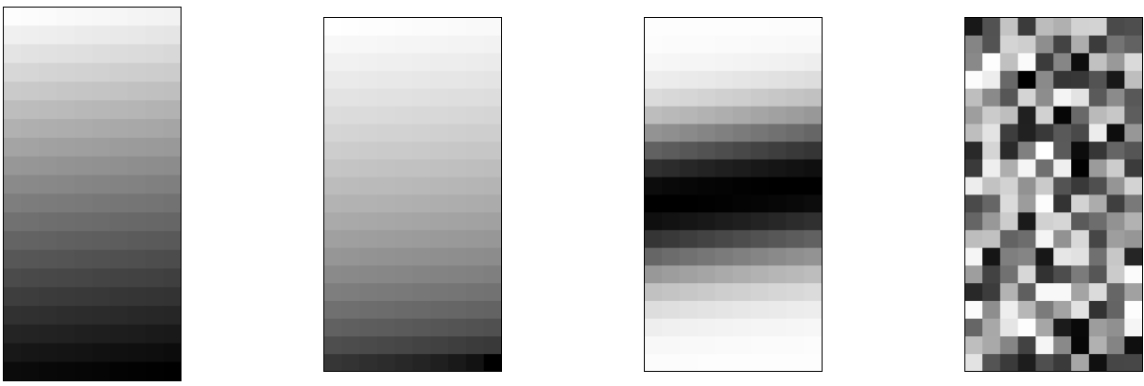
\includegraphics[width=9cm]{img/pixel.jpg}\\
		\vspace*{-0.5em}
		a) Income. \hspace{0.3cm} b) Credit limit. \hspace{0.1cm} c) Transaction volume. \hspace{0.2cm} (d) Age.
	\end{center}

	\note{\textbf{Drawback:} Do not help us to understand the data distribution in a multidimensional space.}
\end{frame}

\begin{frame}{Laying Out Pixels in a Circle Segment Diagram}
	\begin{columns}[t]
		\begin{column}{0.5\textwidth}
			\begin{itemize}
				\item Similar to previous slide but arranged in a circle.
				\item Saves space.
				\item Shows connection among multiple dimensions.
				\item Optionally: Highlight one specific data record as shown opposite.
			\end{itemize}
			\vspace*{1em}
		\end{column}
		\begin{column}{0.5\textwidth}
			\centering

			\begin{tikzpicture}[scale=0.8]
				\pie[hide number]{17/Dim 1, 17/Dim 2, 17/Dim 3, 17/Dim 4, 17/Dim 5, 16/Dim 6}
				\node at (1.5, 1) (a) {\tikzmark{t1} $\circ$};
				\node at (-1.5, 1) (b) {\tikzmark{t2} $\circ$};
				\node at (1.5, -0.9) (c) {\tikzmark{t3} $\circ$};
				\node at (-1.5, -0.9) (d) {\tikzmark{t4} $\circ$};
				\node at (0.1, -1.8) (e) {\tikzmark{t5} $\circ$};
				\node at (0, 1.8) (f) {\tikzmark{t6}$\circ$};
				\node at (-3, 3) (f) {Data record \tikzmark{n1}};
			\end{tikzpicture}
			\begin{tikzpicture}[remember picture,overlay]
				\path[draw=black,thick,-]<1-> (n1) -- (t1);
				\path[draw=black,thick,-]<1-> (n1) -- (t2);
				\path[draw=black,thick,-]<1-> (n1) -- (t3);
				\path[draw=black,thick,-]<1-> (n1) -- (t4);
				\path[draw=black,thick,-]<1-> (n1) -- (t5);
				\path[draw=black,thick,-]<1-> (n1) -- (t6);
			\end{tikzpicture}
		\end{column}
	\end{columns}
\end{frame}

\begin{frame}{Polar Plot}
	\begin{columns}[t]
		\begin{column}{0.5\textwidth}
			\begin{itemize}
				\item Alternative to pixel-oriented or circle segment diagram.
				\item Saves space.
				\item Shows connections among multiple dimensions for each data record.
				\item Downside: Can get crowded with too much data records.
			\end{itemize}
		\end{column}
		\begin{column}{0.5\textwidth}
			\vspace{-5em}
			\begin{center}
				\includegraphics[width=\textwidth,clip, trim=0cm 0cm 0cm 2.6cm]{img/dimension-plot.pdf}
			\end{center}
		\end{column}
	\end{columns}
\end{frame}

\begin{frame}{2. Geometric Projection Visualization Techniques}
	Visualization of geometric transformations and projections of data.

	\textbf{General Methods:}
	\begin{itemize}
		\item Scatter plot and scatter-plot matrices.
		\item Parallel coordinates.
	\end{itemize}

	\textbf{Additional Methods:}
	\begin{itemize}
		\item Projection pursuit\footnote{\fullcite{friedman1974}}.
		      Finds a linear projection (one- or two-dimensional) that are ``highly revealing''.
		\item Prosection views\footnote{\fullcite{furnas1994}}.
		\item Hyperslice\footnote{\fullcite{wijk1993}}.
	\end{itemize}
\end{frame}

\begin{frame}{Scatter Plot Matrices}
	\centering
	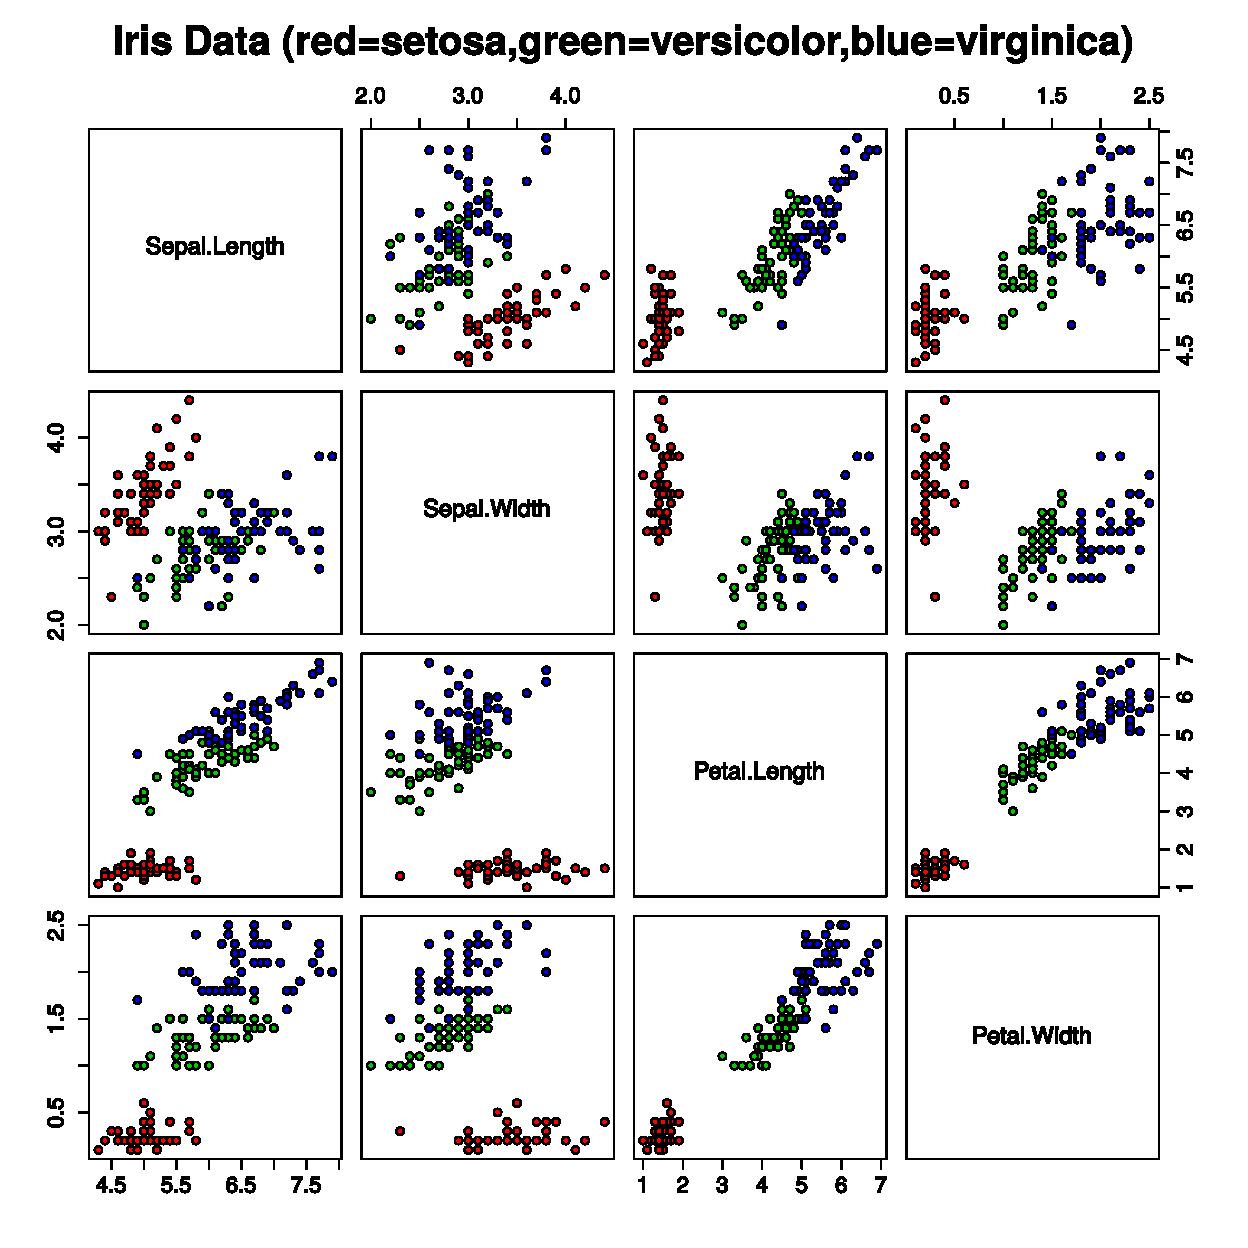
\includegraphics[height=6.5cm]{img/scatterplot_matrix.pdf}
\end{frame}

\begin{frame}{Parallel Coordinate Plot}
	\begin{center}
		\begin{tikzpicture}
			\begin{groupplot}[
					group style={
							group name=iris,
							group size=4 by 1,
							horizontal sep=2cm
						},
					axis y line=left,
					hide x axis,
					width=2cm,
					height=6cm,
					xmin=0,
					xmax=0.5,
					enlarge y limits,
					every axis plot/.append style={opacity=0}
				]

				\nextgroupplot

				\pgfplotsinvokeforeach{0,...,\NumRows} % loop over all rows in table
				{
					% get value in sw column
					\pgfplotstablegetelem{####1}{sw}\of{\iris}%
					% add a coordinate at x=0 and that y-value
					\edef\temp{\noexpand\addplot coordinates {(0,\pgfplotsretval)} coordinate (sl####1);}
					\temp
				}

				\nextgroupplot

				\pgfplotsinvokeforeach{0,...,\NumRows}
				{
					\pgfplotstablegetelem{####1}{sl}\of{\iris}%
					\edef\temp{\noexpand\addplot coordinates {(0,\pgfplotsretval)} coordinate (sw####1);}
					\temp
				}

				\nextgroupplot

				\pgfplotsinvokeforeach{0,...,\NumRows}
				{
					\pgfplotstablegetelem{####1}{pw}\of{\iris}%
					\edef\temp{\noexpand\addplot coordinates {(0,\pgfplotsretval)} coordinate (pl####1);}
					\temp
				}

				\nextgroupplot

				\pgfplotsinvokeforeach{0,...,\NumRows}
				{
					\pgfplotstablegetelem{####1}{pl}\of{\iris}%
					\edef\temp{\noexpand\addplot coordinates {(0,\pgfplotsretval)} coordinate (pw####1);}
					\temp
				}

			\end{groupplot}

			% add labels below
			\foreach \i/\txt in {1/SW,2/SL,3/PW,4/PL}
			\node [below] at (iris c\i r1.south west) {\txt};


			% draw the lines
			% this dataset has three groups of fifty rows each, hence the start/stop values
			\foreach[
				evaluate=\j as \START using int(\j*50),
				evaluate=\j as \STOP using int((\j+1)*50-1),
			] \j/\clr in {0/blue,1/red,2/green}
				{
					\foreach \i in {\START,...,\STOP}
					\draw [color=\clr,opacity=0.5] (sl\i) -- (sw\i) -- (pl\i) -- (pw\i);
				}

		\end{tikzpicture}

	\end{center}
	\textbf{Disadvantage:} Reduced readability when plotting an extensive amount of data records and/or dimensions.
\end{frame}

\begin{frame}{3. Icon Based Visualization}
	\centering
	\begin{itemize}
		\item \textbf{Visualization of the data values as features of icons.}
		\item \textbf{Typical visualization methods:}
		      \begin{itemize}
			      \item Chernoff faces.
			      \item Stick figures.
		      \end{itemize}
		\item \textbf{General techniques:}
		      \begin{itemize}
			      \item Shape coding: \emph{Use shape to represent certain information encoding.}
			      \item Color icons: \emph{Use color icons to encode more information.}
			      \item Tile bars: \emph{Use small icons to represent the relevant feature vectors in document retrieval.}
		      \end{itemize}
	\end{itemize}
\end{frame}


\begin{frame}{Icon Based Visualization: Example}
	\centering
	\includegraphics[width=0.9\textwidth,clip, trim=0cm 0cm 0cm 2.5cm]{img/fau-enrolled-students.pdf}
\end{frame}

\begin{frame}{Chernoff Faces}
	\textbf{Human mind is able to distinguish facial features.} Chernoff faces
	encode multiple dimensions in one face.

	E. g. head eccentricity, eye size, eye spacing, eye eccentricity, pupil size,
	eyebrow slant, nose size, mouth shape, mouth size, and mouth opening.

	\vspace*{1em}
	\begin{columns}[t]
		\hspace*{1.4em}
		\begin{column}{0.6\textwidth}
			\textbf{Disadvantages:}
			\begin{itemize}
				\item Limited power to relate multiple relationships.
				\item Specific features are not shown.
				\item Facial features vary in perceived importance.
				\item Symmetric faces waste space $\rightarrow$ \textit{Asymmetrical } Chernoff
				      faces allows up to 36 dimensions in one face.
			\end{itemize}
		\end{column}
		\begin{column}{0.4\textwidth}
			\vspace*{-2em}
			\begin{figure}
				\centering
				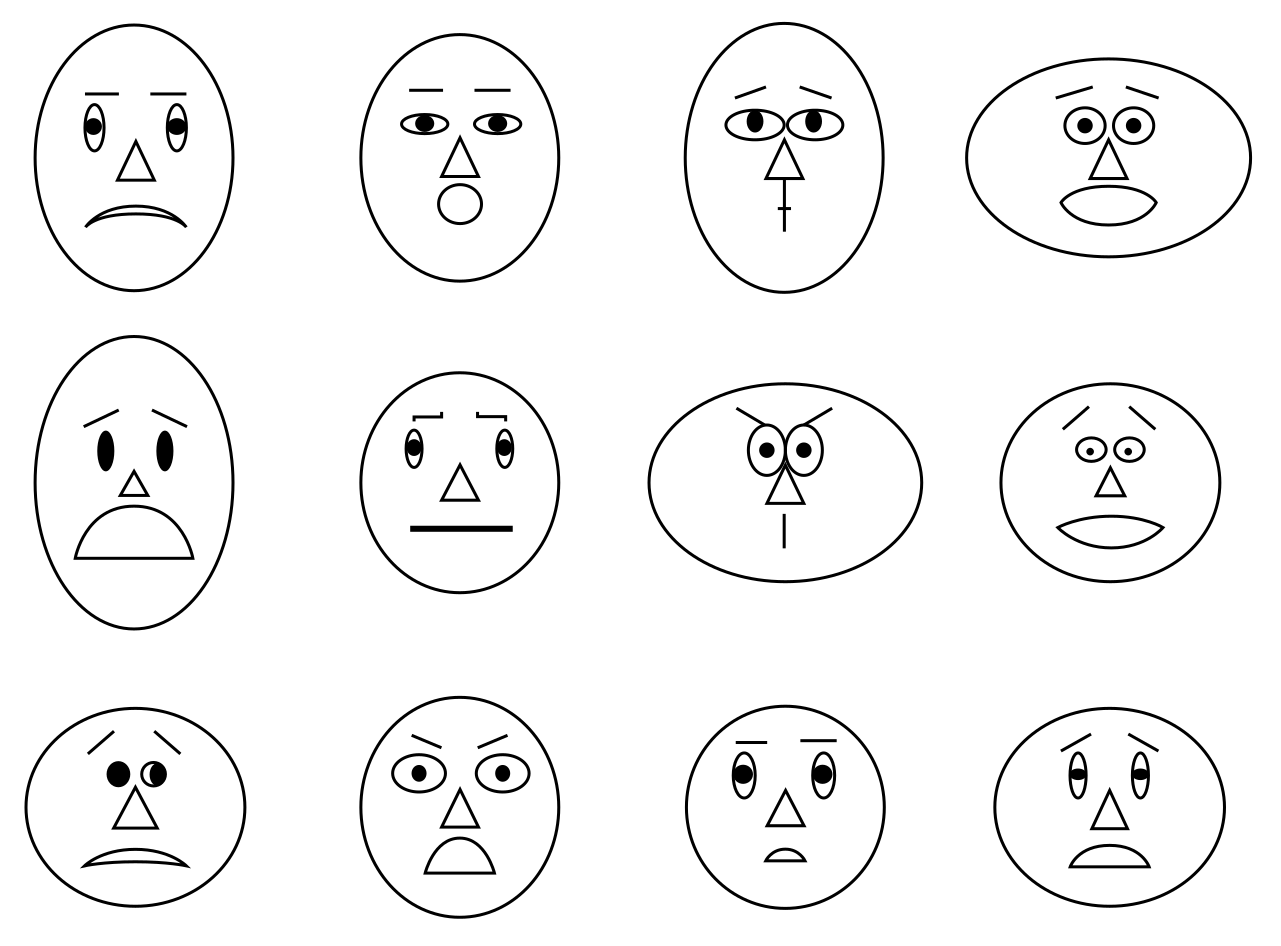
\includegraphics[width=5cm]{img/chernoff_faces.png}
			\end{figure}
		\end{column}
	\end{columns}
\end{frame}


\begin{frame}{4. Hierarchical Visualization Techniques}
	\centering
	\begin{itemize}
		\item \textbf{Visualization of the data using a hierarchical partitioning into subspaces.}
		\item \textbf{Methods:}
		      \begin{itemize}
			      \item Tree maps.
			      \item Cone trees.
		      \end{itemize}
	\end{itemize}
\end{frame}


\begin{frame}{Tree Maps}
	\centering
	\begin{tikzpicture}[xscale = 1.35, yscale = 0.77,
			font=\sffamily,
			mystyle/.style={draw=white, very thick, text=white, font=\sffamily\bfseries},
		]
		\pie[square,
			style={mystyle},
			color={yellow!80!orange, gray, blue!40, orange},
			text=legend,
		]{68/A, 5/B, 5/C, 22/D}
	\end{tikzpicture}
\end{frame}

\begin{frame}{Three Dimensional Cone Trees}
	\begin{itemize}
		\item $3$D cone-tree visualization technique by \citeauthor{robertson1991}\footnote{\fullcite{robertson1991}}:\\
		      works well for up to approx. a thousand nodes.
		\item Build a $2$D circle tree that arranges its nodes in concentric circles centered on the root node.
		\item Overlaps can't be avoided projecting onto $2$D.
	\end{itemize}

	\begin{columns}[b]
		\begin{column}{0.7\textwidth}
			\vspace*{-1em}
			\begin{figure}
				\centering
				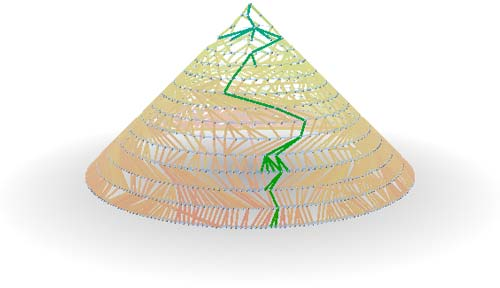
\includegraphics[width=3cm,height=3cm]{img/threedcone_one.jpg}\hspace{1cm}
				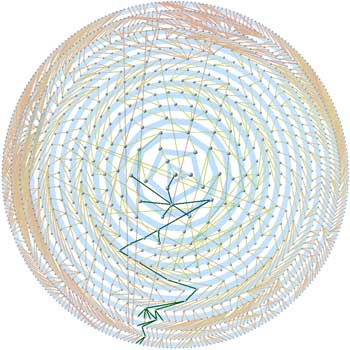
\includegraphics[width=3cm,height=3cm]{img/threedcone_two.jpg}\\
			\end{figure}
		\end{column}
		\begin{column}{0.3\textwidth}
			\tiny{Acknowledgement: \href{ttp://nadeausoftware.com/articles/visualization}{http://nadeausoftware.com/articles/visualization}.}
		\end{column}
	\end{columns}


\end{frame}

\begin{frame}{5. Visualizing Complex Data and Relations}
	\textbf{Visualizing non-numerical data}
	\begin{itemize}
		\item \textbf{Text cloud}
		      \begin{itemize}
			      \item The importance of tag is represented by font size/color.
			      \item Besides text data, there are also methods to visualize relationships, \\ such as visualizing social networks.
		      \end{itemize}
		\item \textbf{Networks}
	\end{itemize}
	% TODO: Add exemplary word cloud and some network
\end{frame}
